\section{Formal Analysis Using Alloy}
In this section a model of the World is provided by the Alloy tool.
\subsection{Model}

\begin{lstlisting}[language=alloy]
open util/boolean

---------------- AVAILABLE PREFERENCES ----------------

sig publicPreference extends Preference {
maxCost : Int,
maxChanges : Int
} { maxCost > 0 and maxChanges >= 0}

sig footPreference extends Preference {
maxDistance: Int
} {maxDistance > 0}

sig bikePreference extends Preference {
maxDistance: Int
} {maxDistance > 0}

sig taxiPreference extends Preference {
maxCost: Int
} {maxCost > 0}

sig carPreference extends Preference {
minDistance: Int
} {minDistance > 0}

sig bikeSharingPreference extends Preference {
maxDistance: Int,
maxCost: Int
} {maxCost > 0 and maxDistance > 0}

sig carSharingPreference extends Preference {
minDistance: Int,
maxCost: Int
} {maxCost > 0 and minDistance > 0}

---------------- AVAILABLE TRANSPORTS ----------------

-- an instance of transport is intended as additional information about a specific travel once the type of mean is defined

sig Foot extends Transport {
distance : Int
} { distance > 0 }

sig Taxi extends Transport {
cost : Int
} { cost > 0 }

sig Car extends Transport {
distance : Int
} { distance > 0 }

sig Public extends Transport {
cost : Int,
nChanges: Int
} { cost > 0 and nChanges >= 0}

sig Bike extends Transport {
distance : Int
} { distance > 0 }

sig carSharing extends Transport {
distance: Int,
cost: Int
} { cost > 0 and distance > 0}

sig bikeSharing extends Transport  {
distance,
cost: Int,
} { cost > 0 and distance > 0}

---------------- MODEL SIGNATURES ----------------

abstract sig Preference {}
abstract sig Transport {}

sig Booking {}

sig User {
calendar: set Schedule,
constraints: set Preference,
id: one Int
} { id > 0 }

sig Schedule {
scheduleEvents: set Event,
scheduleTravels: set Travel
} { 
-- each schedule has 1 starting event i.e. no travel has this event as a destination
-- and 1 final event i.e. no travel has this event as a source, these events can coincide.
-- all other events are connected by travels
(one e: scheduleEvents | no t: scheduleTravels | t.to = e)	and (one e: scheduleEvents | no t: scheduleTravels | t.from = e)
}

sig Event {
start: one Int,
end: one Int,
active: one Bool
} { start > 0 and end > 0 and start < end }

sig Travel {
from: one Event,
to: one Event,
start: one Int,
end: one Int,
mean: one Transport,
travelBooking: lone Booking
} { start > 0 and end > 0 and start < end}

-- each preference is in the constraints of 1 user
fact eachPreferenceBelongsToAUser {
all p: Preference | one u: User  | p in u.constraints
}

-- the id associated with each user is unique
fact userIdsAreUnique {
no disjoint u1, u2 : User | u1.id = u2.id
}

-- each users can specify one constraint/preference of each type
fact userHasOnePreferencePerType {
all u: User {
lone p: Preference | p in bikePreference and p in u.constraints
lone p: Preference | p in footPreference and p in u.constraints
lone p: Preference | p in publicPreference and p in u.constraints
lone p: Preference | p in bikeSharingPreference and p in u.constraints
lone p: Preference | p in carSharingPreference and p in u.constraints
lone p: Preference | p in carPreference and p in u.constraints
lone p: Preference | p in taxiPreference and p in u.constraints
}
}

-- the preferences of each user must be respected in the model
fact preferencesMustBeRespected {
no u: User {
all s: Schedule {
all t: Travel {
some p: publicPreference, pt: Public | pt.nChanges > p.maxChanges and p in u.constraints and t in s.scheduleTravels and t.mean = pt
some p: publicPreference, pt: Public | pt.cost > p.maxCost and p in u.constraints and t in s.scheduleTravels and t.mean = pt
some p: footPreference, ft: Foot | ft.distance > p.maxDistance and p in u.constraints and t in s.scheduleTravels and t.mean = ft
some p: bikePreference, bt : Bike | bt.distance > p.maxDistance and p in u.constraints and t in s.scheduleTravels and t.mean = bt
some p: taxiPreference, tt: Taxi | tt.cost > p.maxCost and p in u.constraints and t in s.scheduleTravels and t.mean = tt
some p: carPreference, ct : Car | ct.distance < p.minDistance and p in u.constraints and t in s.scheduleTravels and t.mean = ct
some p: carSharingPreference, st : carSharing | st.cost > p.maxCost and p in u.constraints and t in s.scheduleTravels and t.mean = st
some p: carSharingPreference, st : carSharing | st.distance < p.minDistance and p in u.constraints and t in s.scheduleTravels and t.mean = st
some p: bikeSharingPreference, st : bikeSharing | st.distance > p.maxDistance and p in u.constraints and t in s.scheduleTravels and t.mean = st
some p: bikeSharingPreference, st : bikeSharing | st.cost > p.maxCost and p in u.constraints and t in s.scheduleTravels and t.mean = st
}
}
}
}

-- each schedule is in the calendar of 1 user
fact eachScheduleBelongsToAUser {
all s:Schedule | one u: User | s in u.calendar
}

-- each active event is in 1 schedule
fact eachEventBelongsToASchedule {
all e: Event | one s: Schedule | e in s.scheduleEvents or (e.active = False and not e in s.scheduleEvents)
}

-- booking is available for public transportation, taxi and sharing services
fact bookingServices {
all t: Travel | all b : Booking | t.travelBooking = b implies t.mean in Taxi + Public + carSharing + bikeSharing
}

-- each travel is in 1 schedule
fact eachTravelBelongsToASchedule {
all t: Travel | one s: Schedule | t in s.scheduleTravels
}

-- each booking referes to 1 travel
fact eachBookingBelongsToATravel {
all b: Booking | one t: Travel | t.travelBooking = b
}

-- each instance of transport is associated with a travel 
fact eachTransportBelongsToATravel {
all tt: Transport | one t: Travel | t.mean = tt
}

-- inactive events do not belong in any schedule
fact inactiveEventsdoNotBelongInAnySchedule {
all s: Schedule | all e: Event | e in s.scheduleEvents implies e.active = True
}

-- for any given travel there are 2 events, source and destination
-- that respectively end before the start of the travel and start after the start of the travel
fact travelIsBetweenEventsTimes {
no t: Travel | t.start < t.from.end or t.end > t.to.start
}

-- each travel must have a source and a destination
fact travelHasToAndFrom {
all t: Travel | some disjoint e1, e2: Event | t.to = e1 and t.from = e2
}

-- no travel can connect events from 2 different schedule
fact noTravelAcrossSchedules {
all t: Travel | all s: Schedule | t.to in s.scheduleEvents implies t.from in s.scheduleEvents and t in s.scheduleTravels
}

-- no travel can connect to or from inactive events
fact noTravelToOrFromInactive {
no t: Travel | t.from.active = False or t.to.active = False
}

-- this means that the instances of the transport are different not the type of transport
fact differentTravelHaveDifferentMean {
no disjoint t1, t2 : Travel | t1.mean = t2.mean
}

-- for each 2 events the start or end time can not coincide
fact scheduleEventsDoNotEndOrStartAtTheSameTime {
all s: Schedule | all disjoint e1, e2: Event | 
(e1 in s.scheduleEvents and e2 in s.scheduleEvents) implies (e1.start != e2.start and e1.end != e2.end)
}

-- events do not intersect
fact noIntersectingEvents {
all s: Schedule | all disjoint e1, e2: Event | 
(e1 in s.scheduleEvents and e2 in s.scheduleEvents and e1.start < e2.start) implies e1.end < e2.start
}

-- there is only one travel that has a certain event as source or as a destination
fact noDoubleTravelPerEvent {
no disjoint t1, t2 : Travel | t1.from = t2.from or  t1.to = t2.to
}
---------------- ASSERTIONS ----------------

-- the event that is not the destination of any travel (starting
assert noEventBeforeFirstAndAfterLastEvent {
all s: Schedule | no disjoint e1, e2 : Event | 
isFirstOfSchedule[e1,s] and e2.start < e1.end and e2 + e1 in s.scheduleEvents or
isLastOfSchedule[e1,s] and e2.end > e1.start and e2 + e1 in s.scheduleEvents
}

-- there are no intersection between schedules in terms of travels and events
assert allSchedulesAreDisjoint {
all disjoint s1, s2: Schedule | no e: Event, t:Travel | (e in s1.scheduleEvents and e in s2.scheduleEvents) 
or (t in s1.scheduleTravels and t in s2.scheduleTravels)
}

-- a travel only connects events in chronological order
assert cannotTravelInThePast{
all s: Schedule | all t: Travel | no e1, e2: Event | (e1+e2 in s.scheduleEvents and t.to = e1 and t.from = e2)
and (e2.end > e1.start)
}

---------------- PREDICATES ----------------

pred show {}

pred isLastOfSchedule[e: Event, s: Schedule] {
no t : Travel | t.from = e and e in s.scheduleEvents and t in s.scheduleTravels
}

pred isFirstOfSchedule[e: Event, s: Schedule] {
no t : Travel | t.to = e and e in s.scheduleEvents and t in s.scheduleTravels
}

pred addEvent[e: Event, s: Schedule] {
s.scheduleEvents = s.scheduleEvents + e
}

pred addBooking[t, t': Travel, new_b: Booking, s: Schedule] {
t'.travelBooking = new_b
t'.from = t.from
t'.to = t.to
t'.start = t.start
t'.end = t.end
t'.mean = t.mean
s.scheduleTravels = s.scheduleTravels - t + t'
t + t' in s.scheduleTravels
}

pred changeEventTime[e, e' : Event, s: Schedule, new_end, new_start : Int] {
e'.start = new_start
e'.end = new_end
e'.active = e.active
s.scheduleEvents = s.scheduleEvents - e + e'
}

pred changeTravelTransport[t, t': Travel, s: Schedule, new_mean: Transport] {
t'.travelBooking = t.travelBooking
t'.from = t.from
t'.to = t.to
t'.start = t.start
t'.end = t.end
t'.mean = new_mean
s.scheduleTravels = s.scheduleTravels - t + t'
t + t' in s.scheduleTravels
}

---------------- CHECK ASSERTIONS ----------------

check noEventBeforeFirstAndAfterLastEvent for  10 Event, 10 Travel, 10 User, 10 Schedule, 10 Transport, 10 Booking, 6 Preference, 4 Int
check allSchedulesAreDisjoint for  10 Event, 10 Travel, 10 User, 10 Schedule, 10 Transport, 10 Booking, 6 Preference, 4 Int
check cannotTravelInThePast for  10 Event, 10 Travel, 10 User, 10 Schedule, 10 Transport, 10 Booking, 6 Preference, 4 Int

---------------- RUN PREDICATES ----------------

run show for exactly 4 Event, 10 Travel, 2 User, 2 Schedule, 10 Transport, 2 Booking,  5 Preference, 4 Int
run addBooking for 10 Event, 10 Travel, 2 User, 2 Schedule, 10 Transport, 2 Booking,  5 Preference, 4 Int
run addEvent for 10 Event, 10 Travel, 2 User, 2 Schedule, 10 Transport, 2 Booking,  5 Preference, 4 Int
run changeEventTime for 10 Event, 10 Travel, 2 User, 2 Schedule, 10 Transport, 2 Booking,  5 Preference, 4 Int
run changeTravelTransport for 10 Event, 10 Travel, 2 User, 2 Schedule, 10 Transport, 2 Booking,  5 Preference, 4 Int

\end{lstlisting}

\subsection{Model Checks}

\begin{figure}[H]
	\centering
	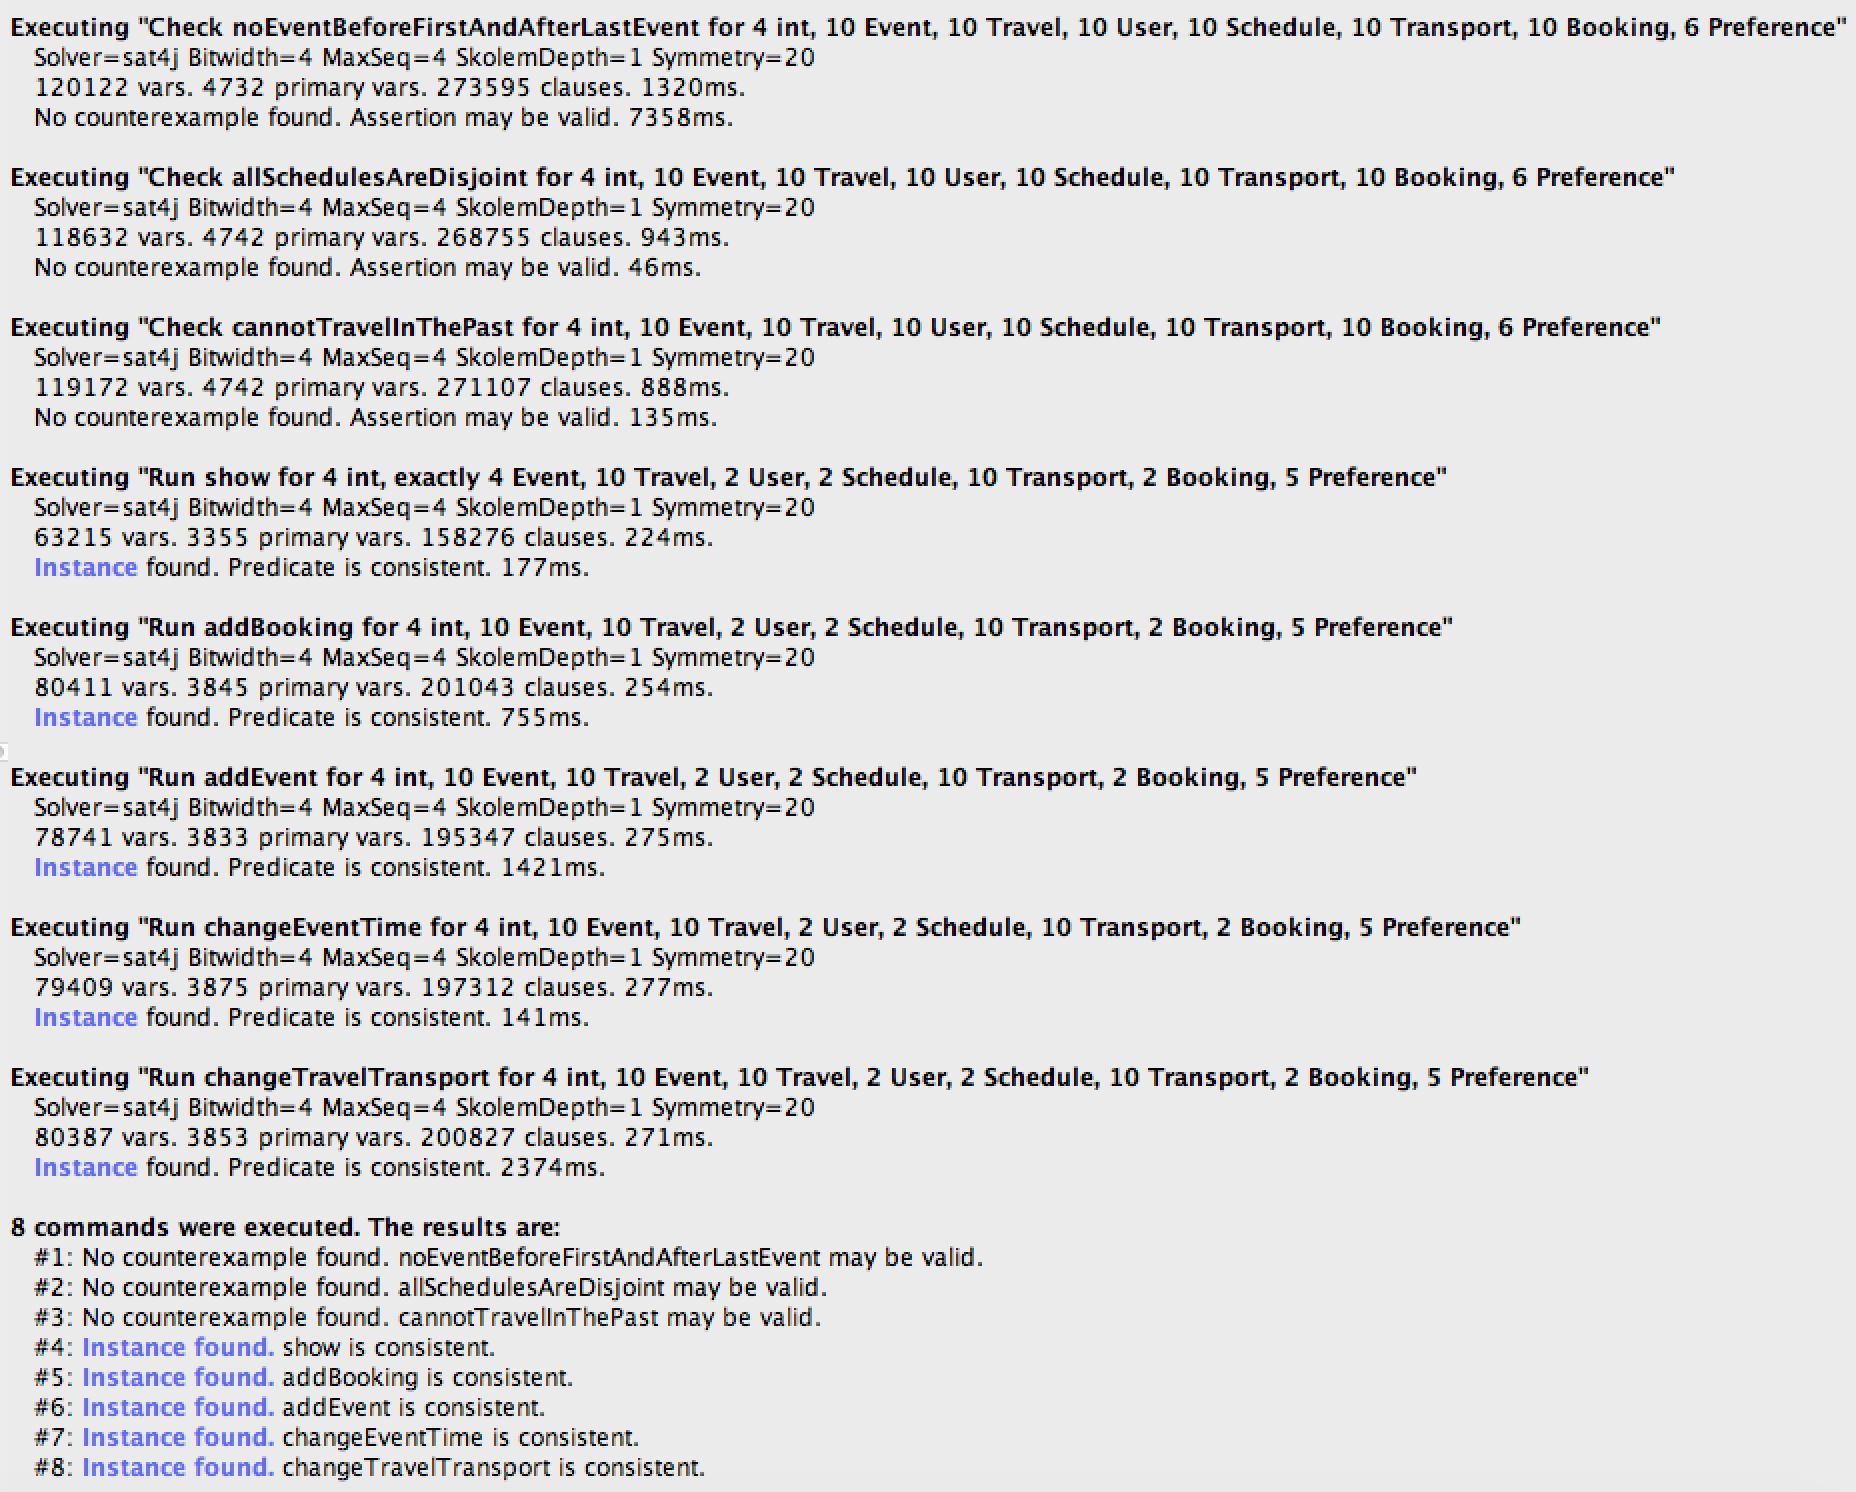
\includegraphics[width=1\textwidth]{res_alloy}
\end{figure}

\newpage

\subsection{Generated Worlds}

\begin{lstlisting}[language=alloy]
pred show {
#Schedule = 1
#User = 1
#Preference = 1
#Booking = 0
}

run show for exactly 2 Event, 10 Travel, 2 User, 3 Schedule, 10 Transport, 2 Booking,  5 Preference, 4 Int
\end{lstlisting}

\begin{figure}[H]
	\centering
	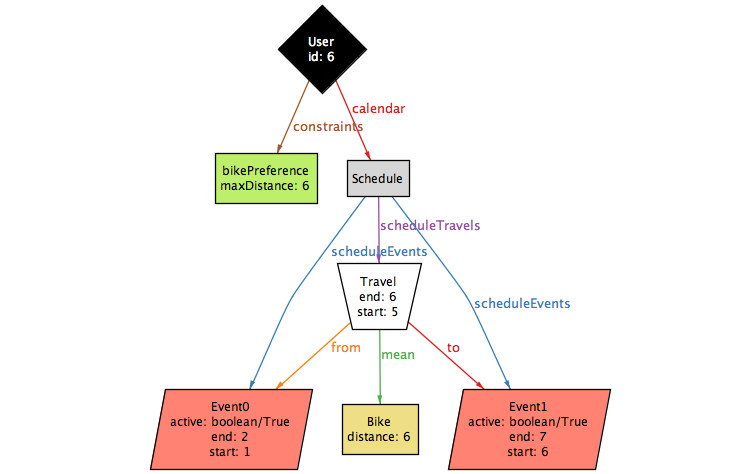
\includegraphics[width=1\textwidth]{world_show_3}
\end{figure}
\newpage
\begin{lstlisting}[language=alloy]
pred show {
#Schedule = 3
#User = 1
#Preference = 2
#Booking = 1
}

run show for exactly 6 Event, 10 Travel, 2 User, 3 Schedule, 10 Transport, 2 Booking,  5 Preference, 4 Int
\end{lstlisting}

\begin{figure}[H]
	\centering
	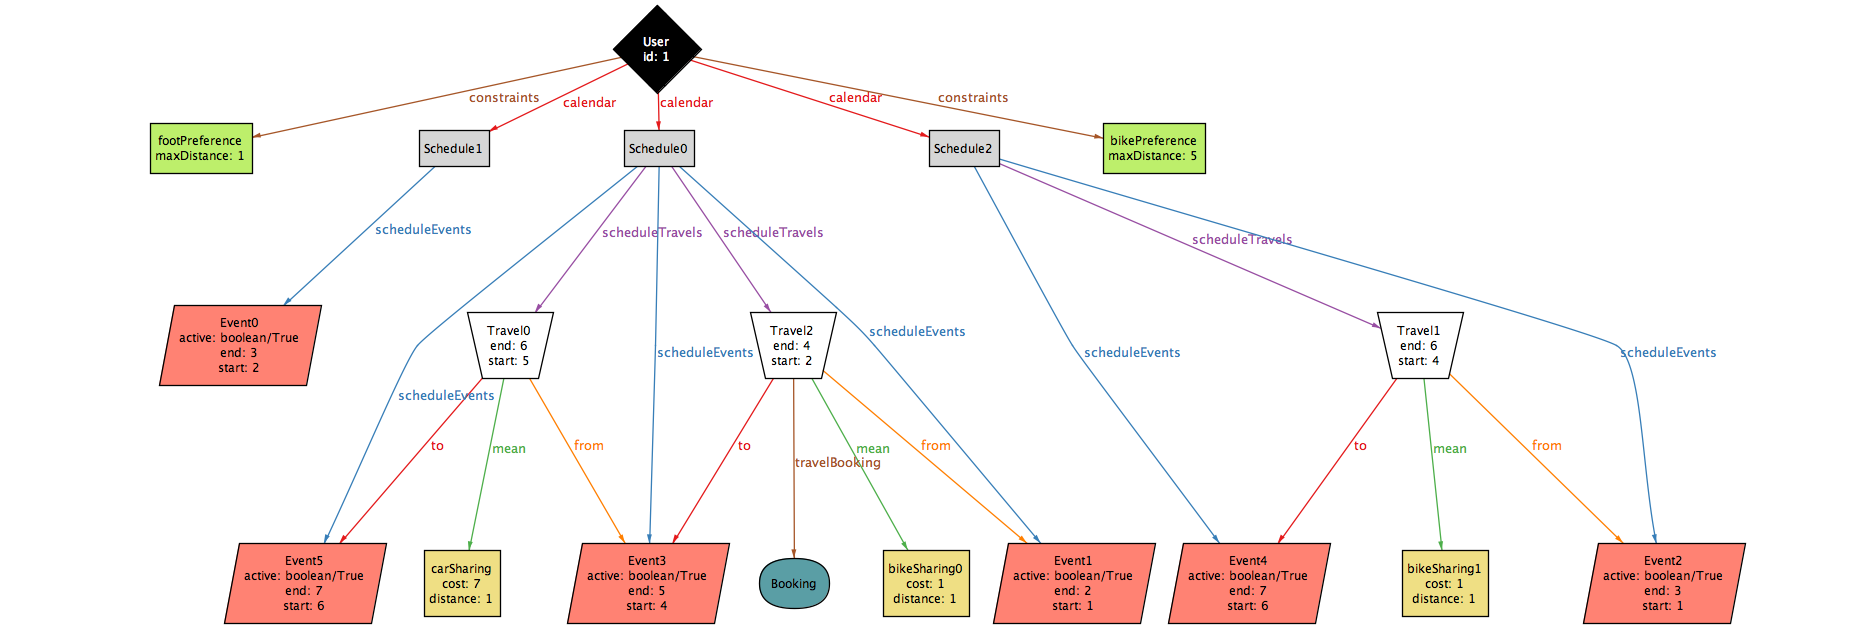
\includegraphics[width=1\textwidth]{world_show_2}
\end{figure}

\begin{lstlisting}[language=alloy]
pred show {
#Schedule = 2
#User = 2
#Preference = 4
#Booking = 1
}

run show for exactly 6 Event, 10 Travel, 2 User, 2 Schedule, 10 Transport, 2 Booking,  5 Preference, 4 Int
\end{lstlisting}

\begin{figure}[H]
	\centering
	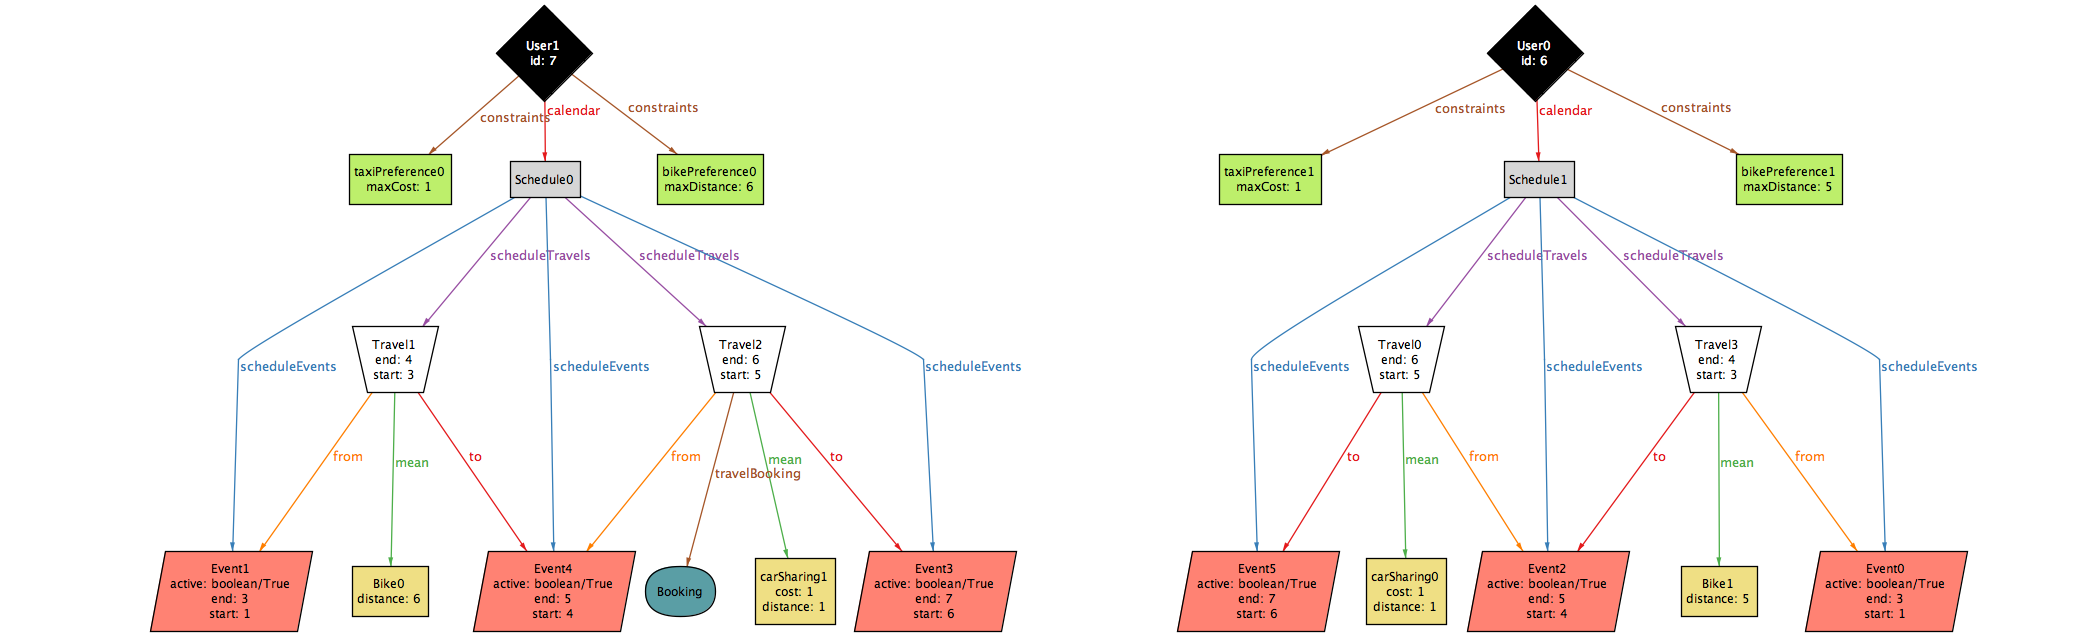
\includegraphics[width=1\textwidth]{world_show_1}
\end{figure}


\begin{lstlisting}[language=alloy]
pred addEvent[e: Event, s: Schedule] {
s.scheduleEvents = s.scheduleEvents + e
}

run addEvent for 10 Event, 10 Travel, 2 User, 2 Schedule, 10 Transport, 2 Booking,  5 Preference, 4 Int
\end{lstlisting}

\begin{figure}[H]
	\centering
	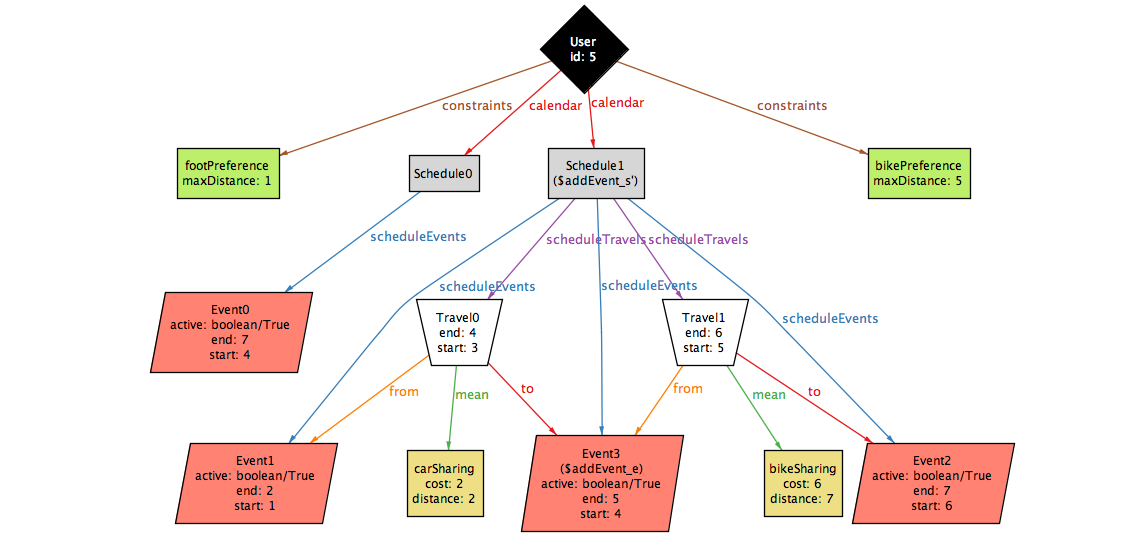
\includegraphics[width=1\textwidth]{world_add_event}
\end{figure}

\begin{lstlisting}[language=alloy]
pred addBooking[t, t': Travel, new_b: Booking, s: Schedule] {
t'.travelBooking = new_b
t'.from = t.from
t'.to = t.to
t'.start = t.start
t'.end = t.end
t'.mean = t.mean
s.scheduleTravels = s.scheduleTravels - t + t'
t + t' in s.scheduleTravels
}

run addBooking for 10 Event, 10 Travel, 2 User, 2 Schedule, 10 Transport, 2 Booking,  5 Preference, 4 Int
\end{lstlisting}

\begin{figure}[H]
	\centering
	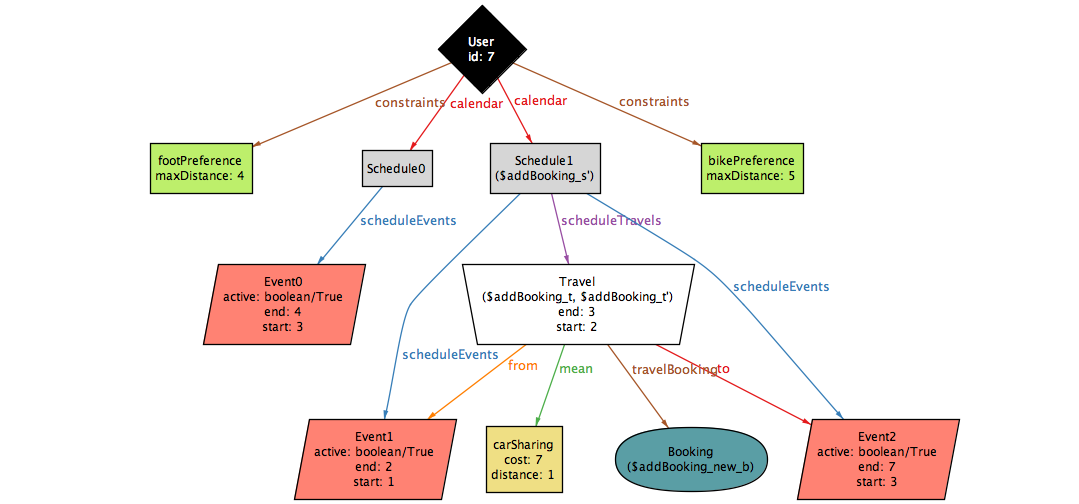
\includegraphics[width=1\textwidth]{world_add_booking}
\end{figure}

\begin{lstlisting}[language=alloy]
pred changeEventTime[e, e' : Event, s: Schedule, new_end, new_start : Int] {
e'.start = new_start
e'.end = new_end
e'.active = e.active
s.scheduleEvents = s.scheduleEvents - e + e'
e + e' in s.scheduleEvents
}

run changeEventTime for 10 Event, 10 Travel, 2 User, 2 Schedule, 10 Transport, 2 Booking,  5 Preference, 4 Int
\end{lstlisting}

\begin{figure}[H]
	\centering
	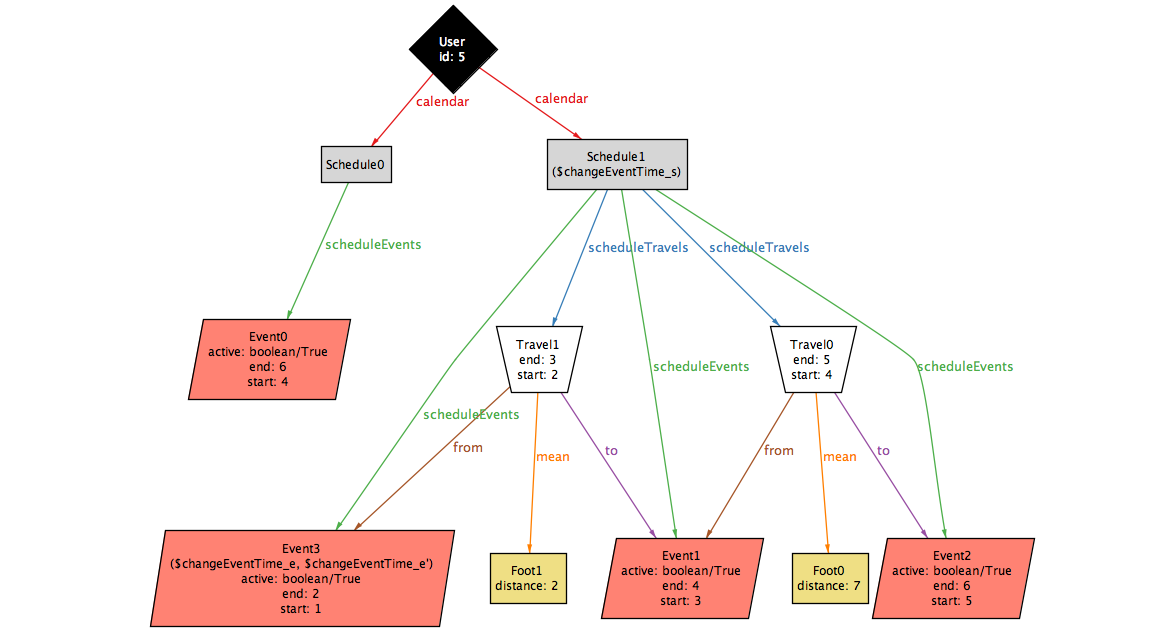
\includegraphics[width=1\textwidth]{world_change_event_time}
\end{figure}


\begin{lstlisting}[language=alloy]
pred changeTravelTransport[t, t': Travel, s: Schedule, new_mean: Transport] {
t'.travelBooking = t.travelBooking
t'.from = t.from
t'.to = t.to
t'.start = t.start
t'.end = t.end
t'.mean = new_mean
s.scheduleTravels = s.scheduleTravels - t + t'
t + t' in s.scheduleTravels
}

run changeTravelTransport for 10 Event, 10 Travel, 2 User, 2 Schedule, 10 Transport, 2 Booking,  5 Preference, 4 Int
\end{lstlisting}

\begin{figure}[H]
	\centering
	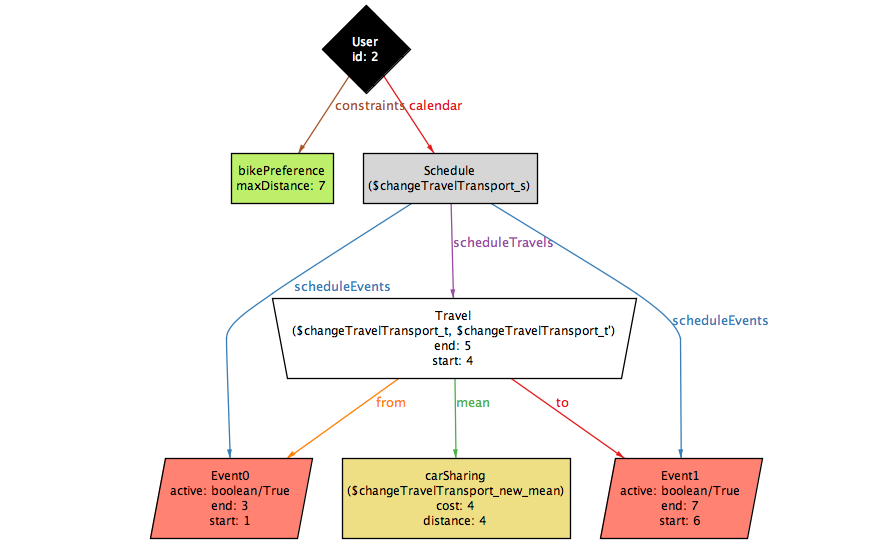
\includegraphics[width=1\textwidth]{world_change_travel_transport}
\end{figure}